% UPAR 2027 Track 1 paper (system v31). WACV 2026 author kit, the format required by the RWS workshop at WACV 2027.
\documentclass[10pt,twocolumn,letterpaper]{article}

%%%%%%%%% PAPER TYPE: anonymous review version (the kit requires a track option in review mode)
\usepackage[review,algorithms]{wacv}
%\usepackage{wacv}  % camera-ready version

%
% --- inline annotations
%
\newcommand{\red}[1]{{\color{red}#1}}
\newcommand{\todo}[1]{{\color{red}#1}}
\newcommand{\TODO}[1]{\textbf{\color{red}[TODO: #1]}}
% --- disable by uncommenting  
% \renewcommand{\TODO}[1]{}
% \renewcommand{\todo}[1]{#1}


\usepackage{booktabs}
\usepackage{amsmath}
\usepackage{graphicx}
\graphicspath{{figs/}}

\definecolor{wacvblue}{rgb}{0.21,0.49,0.74}
\usepackage[pagebackref,breaklinks,colorlinks,allcolors=wacvblue]{hyperref}
\usepackage[capitalize]{cleveref}

\def\wacvPaperID{*****}
\def\confName{WACV}
\def\confYear{2027}

\title{Train Them Together: A Joint Attribute Query over DINOv3 and CLIP\\for Cross-Domain Pedestrian Attribute Recognition}
\author{Anonymous WACV submission}

\begin{document}
\maketitle

%=====================================================================
\begin{abstract}
Pedestrian attribute recognition is trained on some cameras and deployed on others. Two foundation encoders with different pretraining, DINOv3 and CLIP, make different errors under this shift, and the common way to exploit them is to fine-tune each one separately and average their logits. In that scheme neither encoder ever learns what the other one misses. Learning the combination afterwards does not help either: in our experiments every fusion head trained on the frozen features of the two encoders improves on the training domains and loses on the unseen one. We therefore train both encoders in a single model. Each encoder keeps its own attribute query head, and a joint query head lets every attribute attend to the tokens of both encoders at once. The three heads are trained together and averaged at test time, at the inference cost of the two encoders. On a leave-one-dataset-out protocol, the joint model beats the average of separately trained encoders on both held-out datasets in all four runs of the design, and its joint head alone is the best single predictor we trained. Inside the joint head, almost every attention head reads only one of the two encoders, and which one depends on the attribute. With a logit-adjusted loss and a fixed decision threshold of 0.5, the system reaches 0.8001 Challenge\_Avg on the hidden test set of UPAR 2027 Track~1.
\end{abstract}

\begin{figure*}[t]
\centering
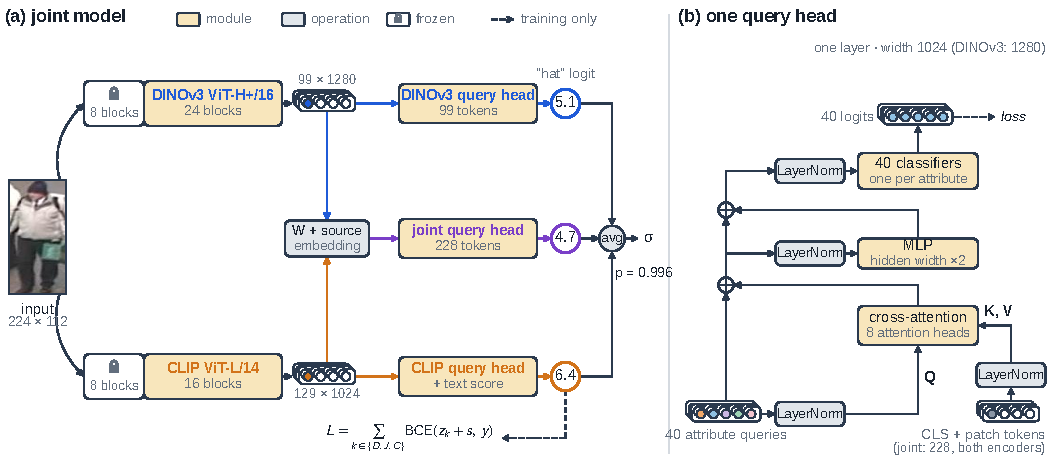
\includegraphics[width=\linewidth]{arch.pdf}
\caption{The submitted model on one PETA image. Both encoders are fine-tuned in one model (hatched blocks are frozen). Besides the query head of each encoder, a joint query head attends to the tokens of both encoders after a linear map to a shared width. The maps show where the ``hat'' query of each head looks, and the circles are the three hat logits that are averaged at test time. Token colors are the first three principal components of the patch tokens. All values come from the submitted weights.}
\label{fig:arch}
\end{figure*}

%=====================================================================
\section{Introduction}
\label{sec:intro}

A pedestrian attribute recognizer meets cameras at test time that it never saw in training. Resolution, viewpoint and lighting change, and each source dataset also labels attributes by its own conventions. The UPAR challenge~\cite{upar,upar24} measures exactly this: models are trained on PA100k~\cite{pa100k}, PETA~\cite{peta} and Market-1501~\cite{market,marketattr} and tested on data from other domains.

Foundation encoders are the strongest starting point for this setting, and two of them complement each other well. DINOv3~\cite{dinov3} is pretrained on images alone and CLIP~\cite{clip} on images with captions, so they fail on different test images. The usual way to use both is to fine-tune each encoder separately and average the logits. Averaging helps, but it fixes the combination before training. Neither encoder is trained to cover what the other one misses, and the combination weights are equal for every image and attribute.

A natural fix is to learn the combination. We tried this on the frozen features of two separately trained encoders, with fusion heads ranging from per-attribute weights to a per-image gate. Every learned head fit the training domains better and the unseen domain worse (\cref{sec:frozen}). The combination learned on frozen features is specific to the source domains.

We therefore move the combination into training (\cref{fig:arch}). Both encoders are fine-tuned in one model. Each keeps its own attribute query head~\cite{q2l,mldecoder}, and a third, joint query head lets each attribute query attend to the tokens of both encoders. The three heads are trained with the same loss and averaged at test time. The joint head is small, so inference still costs two encoder passes. Our findings are:
\begin{itemize}
\item Training the two encoders together with a joint query improves over averaging separately trained encoders on both held-out datasets. The improvement repeats across seeds and design variants and transfers to the hidden test set.
\item The improvement comes from joint training, not from extra parameters. Fusion heads trained on frozen features lose on the unseen domain, and averaging two full systems with twice the encoder passes gains little more.
\item Inside the joint head, almost every attention head reads tokens of only one encoder, and the split between the encoders changes with the attribute.
\end{itemize}

%=====================================================================
\section{Related Work}
\label{sec:related}

\paragraph{Pedestrian attribute recognition.} DeepMAR~\cite{deepmar} cast the task as multi-label classification with frequency-weighted losses. Query-based heads~\cite{q2l,mldecoder} give each label a learned query that cross-attends to the image tokens, and Jia~\etal~\cite{rethinkpar} showed that many earlier architectural gains vanish under a fair split. UPAR~\cite{upar} unified the attribute sets of several datasets into 40 binary attributes, which makes cross-domain evaluation possible.

\paragraph{Combining foundation encoders.} Averaging the predictions of separately trained models is the standard ensemble~\cite{deepens,ovadia}. Distillation methods merge several teachers into one student~\cite{amradio,prism}, which saves inference cost but does not keep the teachers' individual features. Cross-attention between token sets is a common way to fuse modalities~\cite{bottleneck}. We apply it to two image encoders that are trained jointly, and we test it under a domain shift.

\paragraph{Imbalanced attributes.} Most attributes are rare, and the challenge metric weighs positives and negatives of each attribute equally. Logit adjustment~\cite{logitadj} shifts the logits by the log prior during training, so that the raw logits at test time target the balanced error. We use it with DeepMAR weights~\cite{deepmar} and keep a single threshold of 0.5 at test time.

%=====================================================================
\section{Method}
\label{sec:method}

\paragraph{Encoders.} The first encoder is DINOv3 ViT-H+/16~\cite{dinov3} with 840M parameters. The second is the OpenAI CLIP ViT-L/14~\cite{clip} with 303M parameters. Both read a $224\times112$ input with their own normalization. The patch embedding and the first eight transformer blocks of each encoder are frozen, and the remaining blocks are fine-tuned with layer-wise learning-rate decay.

\paragraph{Member heads.} Each encoder has a one-layer query head~\cite{q2l}. Forty learned queries, one per attribute, cross-attend to the CLS and patch tokens with eight attention heads. A residual MLP and a layer norm give one vector per attribute, and a separate linear classifier per attribute turns it into a logit. The CLIP head adds a language score to this logit, as in zero-shot CLIP. The projected CLS token is scored against a text direction per attribute, the CLIP text embedding of a prompt describing the attribute minus that of a neutral prompt. These two heads are the members of our previous submission, where each encoder was trained alone.

\paragraph{Joint query head.} The joint head has the same architecture and reads the tokens of both encoders. A linear layer per encoder maps the 99 H+ tokens (1280-d) and the 129 CLIP tokens (1024-d) to 1024 dimensions, and a learned source embedding is added to all tokens of each encoder. Each of the 40 joint queries then attends to all 228 tokens. Its gradient flows into both encoders, so each encoder is trained in part to supply what the joint queries need. The joint head adds 8.5M parameters.

\paragraph{Training and decision rule.} The three heads are trained with the same loss, and the total loss is their sum. For attribute $a$ with training prior $p_a$, the loss sees each head's logit $z_a$ plus $s_a=\tau\log\frac{p_a}{1-p_a}$, with $\tau=0.32$, inside a binary cross-entropy with DeepMAR weights~\cite{deepmar} and label smoothing of 0.05. Cells that a dataset does not annotate are masked. The shift is applied only in training~\cite{logitadj}. For a rare attribute $s_a$ is negative, so training pushes the raw logit up, and dropping $s_a$ at test time moves the decision toward the balanced error that the challenge metric rewards. At test time the three raw logits are averaged and an attribute is predicted present if the sigmoid of the average exceeds 0.5. The same rule holds for all 40 attributes, and no offset or per-attribute threshold is applied after training.

%=====================================================================
\section{Experiments}
\label{sec:exp}

\subsection{Protocol}
We follow a leave-one-dataset-out protocol. A model is trained on the training split of two source datasets and evaluated on the validation split of the third, which none of its weights has seen. We report the folds that hold out PETA (6,963 test images) and Market-1501 (16,458 images). Each fold trains on 88k to 89k images. We do not report the fold that holds out PA100k, because its training set would have only 18.7k images. The metric is the challenge score Challenge\_Avg, the harmonic mean of the mean balanced accuracy (mA) and the instance F1, in points. Every model uses three epochs, batch size 64, AdamW, an EMA of the weights and bf16. Evaluation uses a single forward pass without flipping, exactly as in the submission. Unless stated otherwise, results are for one training seed.

\subsection{Joint training versus averaging}
\label{sec:main}

\begin{table}[t]
\centering
\small
\setlength{\tabcolsep}{4pt}
\begin{tabular}{@{}lccc@{}}
\toprule
Model & PETA & Market & Mean \\
\midrule
\multicolumn{4}{@{}l}{\emph{Encoders trained separately}} \\
H+ alone & 81.46 & 86.31 & 83.89 \\
CLIP alone & 81.44 & 85.50 & 83.47 \\
Average of the two & 82.45 & 86.30 & 84.38 \\
\midrule
\multicolumn{4}{@{}l}{\emph{Encoders trained together (ours)}} \\
H+ head & 81.31 & 86.17 & 83.74 \\
CLIP head & 81.72 & 85.56 & 83.64 \\
Joint head & 82.10 & \textbf{86.41} & 84.26 \\
Average of H+ and CLIP heads & 82.46 & 86.35 & 84.41 \\
Average of all three heads & \textbf{82.55} & 86.37 & \textbf{84.46} \\
\bottomrule
\end{tabular}
\caption{Held-out Challenge\_Avg (points). Both systems use two encoder passes at test time.}
\label{tab:main}
\end{table}

\Cref{tab:main} compares the two ways of using the encoders. With separate training, the average of the two encoders is clearly better than either encoder alone, which confirms that they are complementary. Joint training changes the members. Taken alone, the H+ and CLIP heads of the joint model are slightly weaker than encoders trained separately, yet their average is already as good as the separately trained pair. The joint head is the strongest single predictor in the table: one head, reading both encoders, comes within 0.12 points of the two-encoder average. Averaging all three heads gives the best result on PETA and the best mean. The gain over the separately trained pair is small, but it is positive on both held-out datasets.

\subsection{Is it joint training or extra capacity?}
\label{sec:frozen}

\begin{table}[t]
\centering
\small
\setlength{\tabcolsep}{4pt}
\begin{tabular}{@{}lcccc@{}}
\toprule
Fusion of frozen encoders & Params & PETA & Market & Mean \\
\midrule
Logit average & 0 & \textbf{82.45} & 86.30 & \textbf{84.38} \\
Per-attribute logit weights & 40 & 82.43 & \textbf{86.31} & 84.37 \\
Classifier on CLIP features & 150k & 81.55 & 86.06 & 83.81 \\
Concatenation + MLP & 155k & 81.27 & 85.92 & 83.60 \\
Per-attribute feature gate & 150k & 81.25 & 85.95 & 83.60 \\
Per-image feature gate & 155k & 81.01 & 85.86 & 83.44 \\
\bottomrule
\end{tabular}
\caption{Learning the combination on frozen features. The heads read the attribute vectors of the two separately trained encoders and add a residual to the averaged logits. They are trained on validation images of the two source datasets, which the encoders never saw, and scored on the held-out dataset.}
\label{tab:frozen}
\end{table}

A joint head adds parameters and a second view of each encoder's tokens. To separate these effects from joint training, we froze the two separately trained encoders and learned the combination on top of them (\cref{tab:frozen}). Each fusion head maps the attribute vectors of both encoders to a correction of the averaged logits. The corrections start at zero, and the loss is the same as in training. We trained the heads on validation images of the two source datasets, so the encoders had never seen their inputs.

None of the learned combinations beats the plain average. Per-attribute logit weights barely move from equal weights, and every feature-based head loses between 0.6 and 0.9 points. The loss is not a failure to fit: on the source-domain images held out from fusion training, the same heads raised the PETA-fold score from 89.2 to about 91.3 points. The fusion heads learn source-specific corrections that do not transfer, and a per-image gate does worst. Joint training avoids this, because the combination and the encoder features are learned on the same data at the same time.

The joint model also comes close to a much larger ensemble. Averaging all five heads of both systems, the separately trained pair and the three heads of the joint model, costs four encoder passes and scores 84.51 points, only 0.05 points above the joint model alone.

\subsection{Variants and seeds}
\label{sec:variants}

\begin{table}[t]
\centering
\small
\setlength{\tabcolsep}{4pt}
\begin{tabular}{@{}lccc@{}}
\toprule
Joint model & PETA & Market & Mean \\
\midrule
Averaged separate encoders & 82.45 & 86.30 & 84.38 \\
\midrule
(a) Submitted model & 82.55 & 86.37 & 84.46 \\
(b) Colour anchors + token dropout & 82.53 & 86.44 & 84.49 \\
(c) (b), second seed & 82.51 & 86.32 & 84.42 \\
(d) (b) + second joint head & 82.51 & 86.43 & 84.47 \\
\midrule
(e) (b) + mid-level tokens & 82.37 & 86.38 & 84.38 \\
(f) (b) + text-initialized queries & 82.23 & 86.48 & 84.36 \\
(g) (a) + flatter clothing attention & 82.39 & 86.35 & 84.37 \\
\bottomrule
\end{tabular}
\caption{Variants of the joint model on the held-out datasets. Runs (a)--(d) keep the design and change details or the seed. Runs (e)--(g) change what the joint head reads or how it attends.}
\label{tab:var}
\end{table}

A gain of this size is close to the run-to-run variation of a single model, so we checked whether it repeats (\cref{tab:var}). Run (b) adds two details to the submitted model. Its CLIP head also scores the colour attributes against dense CLIP patch embeddings, and during training the joint head loses all tokens of one encoder with probability 0.25. Run (c) repeats (b) with another seed, and run (d) gives (b) a second joint head. All four runs (a)--(d) beat the averaged separate encoders on both held-out datasets, eight improvements in eight comparisons. None of the details in (b)--(d) separates clearly from the submitted model.

Runs (e)--(g) show which changes do not help. Adding mid-level tokens to the joint head, initializing the joint queries from CLIP text embeddings, or forcing flatter attention for the 28 clothing queries all lose on PETA and return the mean to the reference level. The useful part is the joint training itself, not a refinement of the joint head.

\subsection{What the joint head learns}
\label{sec:routing}

\begin{figure}[t]
\centering
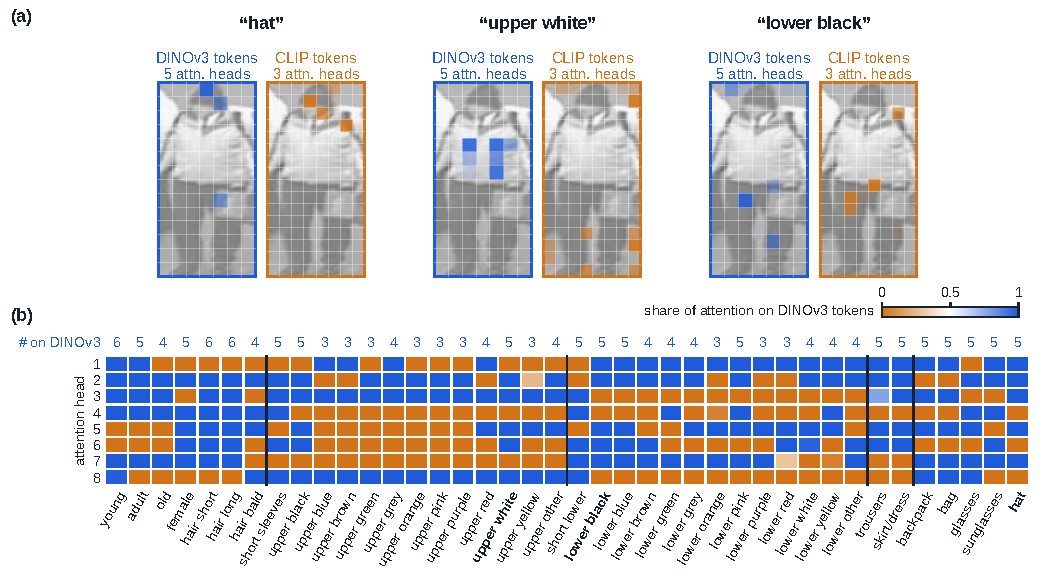
\includegraphics[width=\linewidth]{routing.pdf}
\caption{Attention of three joint queries on the image of \cref{fig:arch}, shown separately for each of the eight attention heads. Each head is drawn on the patch grid of the encoder it reads, and its number is colored by that encoder. The same head can read different encoders for different attributes.}
\label{fig:routing}
\end{figure}

The joint head could mix tokens of both encoders within each attention head, but it almost never does. On the image of \cref{fig:arch}, 312 of the 320 pairs of attention head and attribute put more than 99\% of their weight on the tokens of one encoder, and the remaining eight still put at least 71\%. Which encoder a head reads is not fixed. It changes with the attribute, and the number of heads that read H+ tokens ranges from three to six across the 40 attributes. \Cref{fig:routing} shows three attributes. For the hat, four H+ heads attend to the top of the head, and the CLIP heads attend to the face just below it. For the white top, the H+ heads attend to the jacket, while the CLIP heads attend to a few tokens at the image border. For the black lower body, both encoders are read mostly on the legs and hips. Each attribute query thus divides its attention heads between the two encoders in its own proportion, which a fixed average of two logits cannot do.

The joint head also attends to wider regions than the H+ member. Over 512 PETA validation images, a colour query of the H+ head places 0.88 of its attention on its strongest token on average, while a colour query of the joint head places 0.67. Wider attention alone does not explain the gain, since forcing it in run (g) of \cref{tab:var} did not help.

\subsection{Hidden test set}
\label{sec:test}

\begin{table}[t]
\centering
\small
\setlength{\tabcolsep}{4pt}
\begin{tabular}{@{}lc@{}}
\toprule
Submission & Challenge\_Avg \\
\midrule
Separate encoders, weighted BCE & 0.7893 \\
Separate encoders, logit-adjusted loss & 0.7989 \\
Joint model, logit-adjusted loss (ours) & \textbf{0.8001} \\
\bottomrule
\end{tabular}
\caption{UPAR 2027 Track 1 hidden test. All three submissions use DINOv3 ViT-H+ and CLIP ViT-L, two encoder passes per image and a fixed threshold of 0.5. Final models are trained on the training and validation splits of all three datasets.}
\label{tab:test}
\end{table}

\Cref{tab:test} reports our submissions on the hidden test set. The logit-adjusted loss lifts the separately trained pair by about one point at the same threshold, because it raises the raw logits of rare attributes. Joint training then adds 0.12 points, in line with the gain measured on the held-out datasets. The final model runs at 3.04\,ms per image on an RTX 5090, within the challenge budget of five minutes per run on an A10 GPU.

%=====================================================================
\section{Conclusion}
\label{sec:conclusion}

Two complementary foundation encoders are usually combined after training. We find it better to combine them during training. A joint query head that reads both encoders, trained together with each encoder's own head, improves on the average of separately trained encoders on both held-out datasets in every run of the design, at the same inference cost. Learning a combination on frozen encoders fails under domain shift, which locates the benefit in joint training. Inside the joint head, nearly every attention head reads one encoder per attribute, so different attributes take different shares of the two encoders. The measured gain is modest, and testing whether it grows with more diverse source domains is the natural next step.

{\small
\bibliographystyle{ieeenat_fullname}
\bibliography{refs}
}

\end{document}
